\documentclass{sbir}

\fxsetup{
    status=final,
    author=Lambrinski,
    layout=margin,
    theme=color,
    targetlayout=color
}

\addbibresource{bib/common.bib}
\addbibresource{bib/references.bib}

%%%%%%%%%% Proposal-specific Information %%%%%%%%%%%%%%%%
\company{Damour Systems, PBC}
\proposaltitle{ORACLE: Learning Analytics and Prediction}
\topicnum{AF17A-T009}
\proposalnum{AF17A-T009-1629}
\proposaltype{STTR Phase I Proposal}
%%%%%%%%%%%%%%%%%%%%%%%%%%%%%%%%%%%%%%%%

\begin{document}

%%%%% List the FiXme annotations  %%%%%
%\listoffixmes
%\newpage

%%%%%  Roman numerals for TOC  %%%%%
\pagenumbering{roman}
% \tableofcontents
% \newpage

%%%%% Set the page number that the main proposal will start on %%%%%%
\pagenumbering{arabic}
\pagestyle{proprietary}

\cfoot{
{\color{LeTigre}\vspace*{-1.1in}{\it\small{This proposal includes data that shall not be disclosed outside the Government and shall not be duplicated, used, or disclosed-in whole or in part-for any purpose other than to evaluate this proposal. If, however, a contract is awarded to this offeror as a result of – or in connection with – the submission of this data, the Government shall have the right to duplicate, use, or disclose the data to the extent provided in the resulting contract. This restriction does not limit the Government's right to use information contained in this data if it is obtained from another source without restriction. The data subject to this restriction are contained in pages 1--6 and 8--20.}~\\
\scshape\fromproposaltitle}~\\ \rm\thepage }
}

\sbirsection{Identification and Significance of the Problem or Opportunity}
{The AHS team proposes to develop and deliver a functional prototype system, hereafter termed CHAMELEON, coupled with a reference architecture demonstrating moving target/dynamic defenses (MTD/DD) via network address randomization, integrated intrusion detection and prevention, multi-path encrypted packet transfer, and incorporated secure naming. This system leverages our expertise in software defined networking (SDN), network functions virtualization (NFV), usage management and policy-centric information networks, builds on our previous work under the NUBLU STTR grant in which we have implemented rapid enclave formation and malicious node excision using COTS hardware via established SDN controller software using NFV techniques.}

%%%%%  Evaluation Criteria box, use \begin{evalbox} \end{evalbox}, \evalhdr, \begin{evalitemize}, and \end{evalitemize}  %%%%% 	
\begin{evalbox}
\evalhdr{Innovative:}
  \begin{evalitemize}
     \item Addresses network address randomization using a proven software infrastructure.
     \item Underlying framework supports IDS/IPS and service management capabilities.
  \end{evalitemize}
\evalhdr{Sound Technical Approach:}
  \begin{evalitemize}
     \item Based on open standards and open source product development.
     \item Leverages UNM and AHS's demonstrated work SDN/NFV and usage management.
  \end{evalitemize}
\evalhdr{Qualifications:}
  \begin{evalitemize}
     \item One AHS co-PI has significant experience with SBIR/STTR development and technology transition.
     \item Another AHS co-PI has considerable expertise in information security and usage management.
     \item AHS scientist has extensive knowledge of SDN/NFV, MTD/DD, and software engineering and architecture.
  \end{evalitemize}
\evalhdr{Benefits:}
  \begin{evalitemize}
     \item Hides information flow and network topology, and increases attacker's cost.
     \item Incorporates sophisticated network IDS/IPS sensors.
     \item Rapidly deploy and tear down computational services and enclaves.
%     \item Increase costs to attackers.
  \end{evalitemize}
\evalhdr{Commercialization:}
  \begin{evalitemize}
     \item Will leverage Innovate ABQ.
     \item Deployable in multiple industries with sensitive information.
     \item Uses technologies currently being deployed in data centers.
  \end{evalitemize}
\end{evalbox}

\paragraph{Executive Summary}
\paragraph{The Problem.} 
Today it is widely accepted that cyber-warfare asymmetrically favors the attacker.  While network defenders are required to defend thousands of systems, attackers only need to find a single flaw. As a result of this essential asymmetry, organizations have been actively looking into methods through which defenders can increase the cost of compromise to attackers. One of the approaches the academic community is actively researching is network address randomization, an approach through which systems and services are randomly moved from address to address via a large address space. This approach has had remarkable success in some cases, but has yet to be widely distributed into commercial networks~\cite{AnAkPe:07}.

\vspace*{-0.05in}
The goal of this SBIR effort is to implement a network address randomization system that can effectively randomize addresses, hide overall network topology and traffic volumes, and support excision of compromised nodes, all without negatively impacting overall system performance. This system will also provide facilities for rapid enclave setup and teardown, support robust encryption, and run on commercially available hardware. {\bf Our proposed system, CHAMELEON, will extend our current NUBLU framework.  The NUBLU framework already supports enclave management, robust encryption, and runs on commercially available hardware. It also has an extensible underlying technical architecture with all the primitive functionality required to support network address randomization and overall network traffic obfuscation.} By extending NUBLU, we can focus our efforts on randomization algorithms, secure naming, and traffic shaping algorithms without needing to focus on developing any underlying technology. 

\vspace*{-0.05in}
This technology meets the goals of the SBIR and provides support for not only the requirements of the call, but the desired attributes as well.  Additionally, the NUBLU framework provides additional policy-based usage management capabilities that can provide guaranteed levels of security within deployed enclaves.

\vspace*{0.1in}
\hrule

\clearpage
\cfoot{\color{LeTigre}\vspace*{-1.25em}{\scshape\fromproposaltitle}~\\ \rm\thepage~\\ 
\it{Use or disclosure of data contained on this page is subject to the restriction on the first page of this volume.}}

\paragraph{The Solution Objective.} The AHS Team, composed of personnel from AHS Engineering Services, personnel affiliated with the University of New Mexico (UNM) and Cohesive Integrations, proposes to design, prototype, and develop CHAMELEON, a network randomization system. CHAMELEON will extend our NUBLU framework, a highly flexible usage-managed information-centric network built to protect information transmitted through dynamically configured information domains. NUBLU has been used in standalone configurations and integrated with both cloud computing infrastructures and other widely used computer network systems. Our objective is to extend our current technology to provide network address randomization, intrusion detection/protection system (IDS/IPS) sensors to detect network reconnaissance, and network traffic and topology obfuscation without negatively impacting overall quality of service.

\paragraph{Our Approach.} Our enclave deployment capabilities have already been developed in the scope of NUBLU, as has our ability to support various encryption protocols. The NUBLU enclaves are based on a virtual machine (VM) processing fabric with in-process service containers. We also have the control and management framework in place for these various capabilities. With this already in place, we will immediately begin extending our management components, both local and distributed, to support address randomization and multipath packet routing. We will additionally begin work on a parallel track to keep a local domain name system (DNS) synchronized with randomized address changes. For Phase I we will not attempt to authenticate or keep DNS traffic confidential, nor will we begin work on specific traffic obfuscation algorithms---rather, we will lay the appropriate groundwork for this to commence in Phase II. We will also not begin work with various IDS functions until Phase II, instead focusing on core functions as described in the SBIR topic call.

\paragraph{Vision and End-State.} At the end of Phase I, we will deliver a proof-of-concept of the CHAMELEON system. This system will demonstrate multipath traffic management, network address randomization, a robust enclave creation and management capability, and robust encryption. We will furthermore have conducted initial work to understand the specific impacts of various randomization algorithms on overall quality of service and outlined the design for both authenticated and confidential Domain Name System Security Extensions (DNSSec) extensions and IDS/IPS functionality around honeypots and local network telescopes.

\sbirsection{Phase I Technical Objectives}
{CHAMELEON is a dynamic network address randomization system that provides enhanced cyber-security to protected systems via overall network topology manipulation, dynamic deployment, and secured communication.}

In order to meet the project objectives we propose to extend the technology we developed under the NUBLU STTR grant to incorporate network address randomization, network telescope capabilities~\cite{MoShVo:04}, and automated honeypot deployments~\cite{honeypot}. The technology we have developed currently supports strong encryption of data flows at the Internet layer via Internet protocol security (IPsec) and the application layer via transport layer security  (TLS). It also provides capabilities for fast enclave setup and teardown via OpenFlow~\cite{openflow1.4} and Docker~\cite{docker}.

We intend to add address randomization using software defined networking (SDN) techniques via our existing infrastructure, using OpenDaylight~\cite{opendaylight} as our primary controller technology. We will extend Jararian's approach~\cite{JaAlDu:12}, incorporating Docker's address mapping capabilities~\cite{docker}, to provide robust randomization of network targets.

\begin{figure}[!t]
\centering
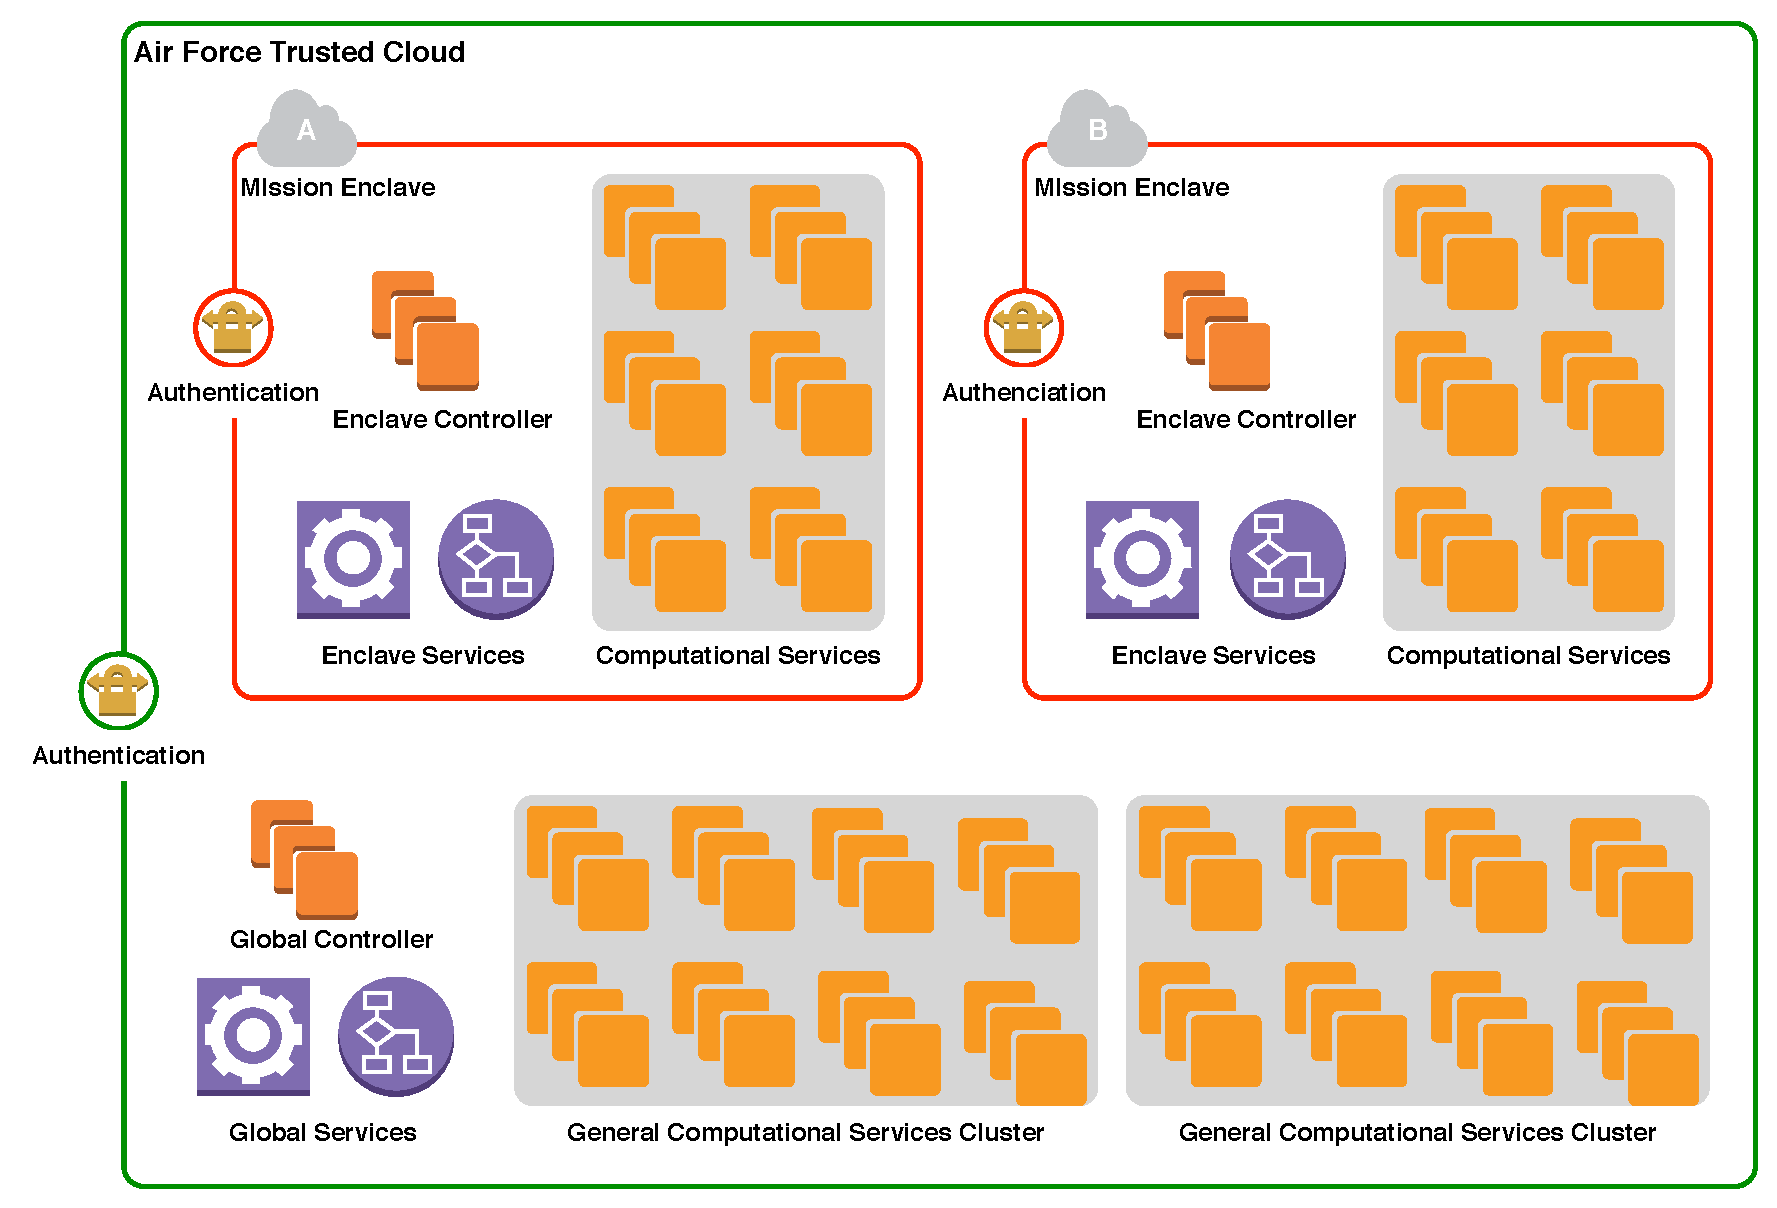
\includegraphics[width=\textwidth]{images/conops.pdf}
\caption{The overall concept of operations of the CHAMELON system, highlighting enclave creation, from a logical perspective.}
\label{fig:conops}
\end{figure}

Figure \ref{fig:conops} shows the overall logical operation of the proposed system.  We envision the system as a whole to run a common computational infrastructure, such as  milCloud or a virtual private cloud hosted at Amazon.  This would form an underlying infrastructure of computational and service resources required to provide various services to internal and external clients.  Overall, the entire system would use network address translation (NAT) to provide a large, private address space in which to distribute services (and increase the overall entropy of the system, making it more difficult for attackers to stumble on randomized service endpoints).  Services are hosted within Docker containers hosted within a scalable VM fabric. The use of in-process virtualization via Docker combined with hypervisor virtualization effectively separates service scaling from computational scaling. Moving an in-process image can happen on the scale of fractions of a second, while effectively spinning up and configuring a new hypervisor image generally takes minutes. Separating services from virtual machines in this way allows us to use different algorithms to predict needs for service as opposed to computation scaling.  In-process virtualization furthermore gives us the ability to frequently recycle running services with fresh images, further decreasing the attack surface of deployed systems.

Each enclave has a redundant OpenDaylight controller, as does the overall global system.  This provides enhanced isolation for enclaves with failover capability to the global controller if needed.  Key enclave and global services include secure naming, public key infrastructure (PKI), and systems for collecting address space monitoring information.  Secure naming services extend DNSSec with custom extensions providing confidential communications and query authentication and authorization.  PKI endpoints provide typical PKI services, including certificate revocation lists and online certificate status protocol (OCSP) services.  Address space monitoring systems collect data from all deployed Openflow switches and controllers on non-routed traffic checking for port scanning or attempted unexpected access of systems at previously allocated addresses, essentially implementing stateful, protocol-aware firewalls at every network switch.

\begin{figure}[!t]
\centering
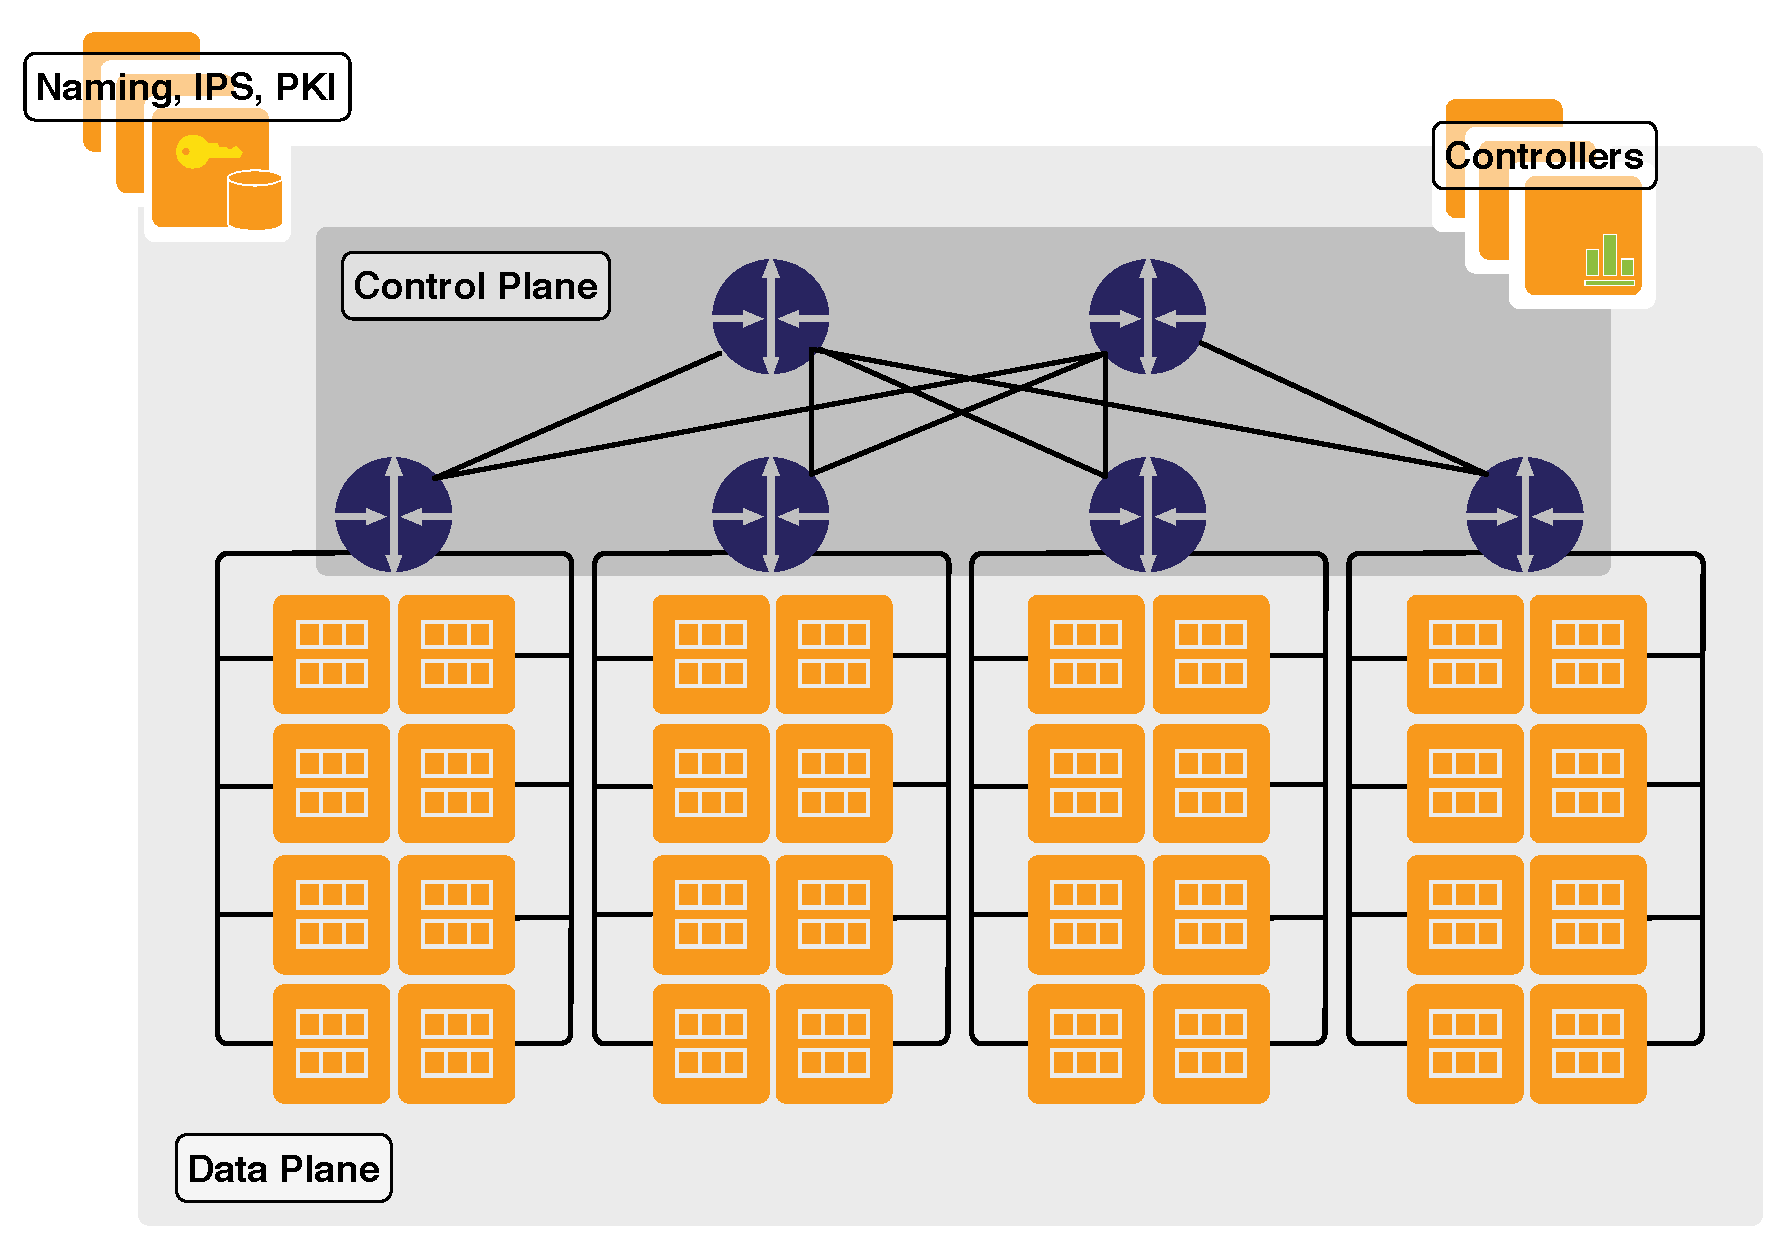
\includegraphics[width=\textwidth]{images/physical.pdf}
\caption{A logical/physical representation of the proposed system including Docker containers and supporting services.}
\label{fig:physical}
\end{figure}

Figure \ref{fig:physical} shows a physical perspective of our laboratory, divided into racks and switching infrastructure we have in place to support CHAMELEON development.  General services, like naming, PKI, and intrusion detection are available to all containers and virtual machines. The logically distributed controller system focuses on both the network control plane, submitting flow information to all connected switches, and the general data plane, handling container motion throughout the virtual machine processing fabric. It manages all network address randomization as well.

\begin{figure}[!t]
\centering
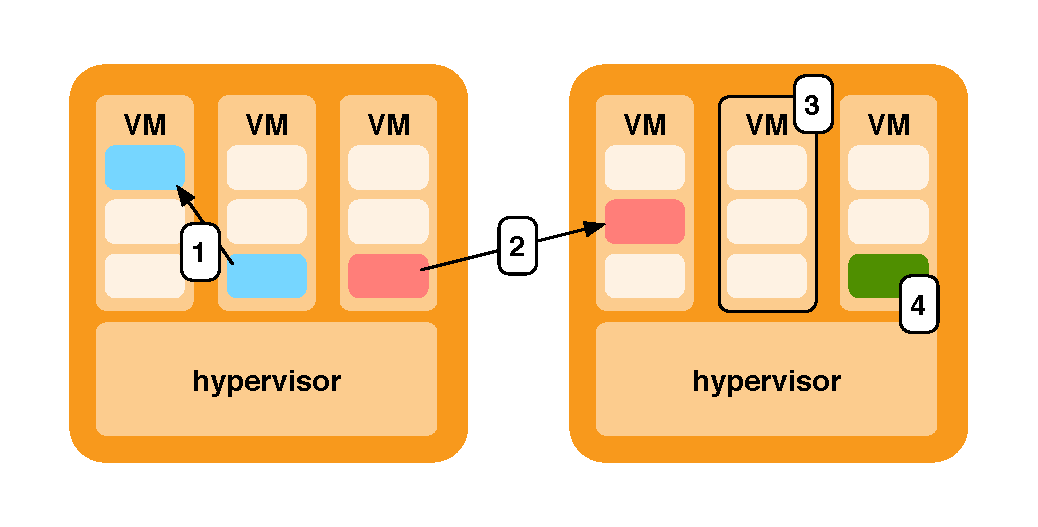
\includegraphics[width=\textwidth]{images/fabric.pdf}
\caption{Use cases associated with the processing fabric of the CHAMELEON system, comprised of virtual machines running on hypervisors via OpenStack containing Docker in-process containers.}
\label{fig:fabric}
\end{figure}

Figure \ref{fig:fabric} shows some of the typical use cases for the system. In case (1), a Docker container from one virtual machine is transferred to another within the same physical system. Here, not only was the container transferred within the processing fabric, but the address information was also changed.  Case (2) shows the same operation between physical systems. Removing a compromised node is an extension of Case (2).  Case (3) highlights changing the address information associated with an entire virtual machine image, while case (4) demonstrates changing address information with a single hosted docker container.  Technology developed via the NUBLU grant provides functionality associated with cases (1) and (2) today (including node excision).  Cases (3) and (4) would be developed within our existing technology framework via this grant.

The primary focus of this project is to establish a viable network-centric moving-target defense system based around network address and data flow randomization and obfuscation.  This area has been actively researched for roughly the past decade, through work primarily funded by DARPA~\cite{KeFiLo:01}. The goal of this work is to take the current state of the art, move it into production systems, and by doing so increase the cost to attackers to breach those systems while maintaining current operations for legitimate users.

\paragraph{Increase attacker cost and risk.}
{\bf The overarching goal of this project is to increase the cost of malicious system reconnaissance by shrinking the time window over which collected information is valid}.  This increases attacker cost and risk in two specific ways. First, deployed software cannot be configured to use static resource lists previously collected through covert means. Second, because of this inability to use previously collected information, deployed malicious payloads must incorporate enough intelligence to analyze as well as attack identified infrastructure.  The former increases overall risk of deployment and detection, while the latter significantly increases payload development costs.

\paragraph{Network topology mis-representation.}
We will use network address space randomization (NASR)~\cite{KeFiLo:01,AtPaWe:03,AnAkPe:07} and host motion via software defined networking (SDN)~\cite{JaAlDu:12} and network functions virtualization (NFV) as the primary mechanism through which we will hide the logical structure of a computer network.  Generally, NASR randomizes ports and addresses of a communication network over some previously selected time interval and uses either an oracle or a known algorithm with a secret seed to allow systems to predict the current addresses of needed services. So far, these approaches have been applied to more traditional Internet Protocol (IP) networks rather than industrial control system or mobile ad-hoc networks.

We will use an oracle-based approach via SDN controllers and the management infrastructure developed under the NUBLU grant.  We will begin with the approach outlined by Jafarian et. al. ~\cite{JaAlDu:12} in a simulated environment. {\bf Our focus will be on the potential use of this approach within our framework in an operational environment with real traffic and strict quality-of-service rather than a notional network, and the direction of our initial development will reflect that.} Specifically, we will begin our simulations with much larger network using more realistic topologies, in both Mininet and Internet2 environments. We will be looking closely at the effect of randomization on overall quality-of-service and usability, key concerns in CHAMELEON moving forward. We will use open standards in this work to enforce control of the network enabling us to easily move from simulated to real environments.

\paragraph{Data flow obfuscation.}
Hiding the true logical topology via NASR is not sufficient to hinder network mapping efforts. Services can still be identified by tracing traffic origins back to the current randomized IP address and port by attackers with network access. In order to sufficiently hide the service profile and logical topology of a network, we must also camouflage the volume and direction of transmitted data. Random host motion coupled with address and port randomization will address the later requirement, while multipath packet routing addresses the former.

{\bf We will manage multipath routing via SDN as well.} This will of course have direct impacts on underlying physical network design, as the networks over which we implement CHAMELEON must be able to support multiple routes between hosts.  SDN approaches are well suited to this however, in that we will have fine-grained programmatic control over the switching fabric of target networks.

\paragraph{Prevent traffic analysis.}
Generally, IP traffic can be analyzed via netflow or full packet information.  Ideally we will hide the traffic flowing across the network from malicious actors.  Full packet information can be effectively hidden with encryption.  Netflow information is more difficult to hide, but appropriate NASR will greatly lessen the risk represented by acquired netflow data by reducing its window of validity and by doing so its value as well.

{\bf Our proposed SDN approach allows us to manipulate host locations, addresses, and traffic flow, greatly increasing the difficulty of network traffic analysis.} In this kind of a system, service containers are moving from host to host, the addresses of those containers are constantly changing, and traffic that could be used to track those containers is encrypted and routed over multiple paths through the network. All of this can be randomized, and over an appropriately large address space, this makes network reconnaissance very difficult.

\paragraph{Rogue client prevention, detection and excision.}
By deploying systems and randomizing address information over a large address space and actively monitoring the remainder, we can use the unused address space at any point in time as a local network telescope. We can detect scanning activity, and preferentially weight any connection attempts to addresses previously used by services with randomized addresses. Our heavily virtualized infrastructure furthermore allows us to deploy preconfigured honeypots as virtualized network functions we can use to attract, contain, and monitor any malicious activity. {\bf As our NUBLU system already provides for compromised node removal, in this effort we can focus efforts on novel IDS/IPS sensors.}

\paragraph{Minimal service impact with COTS hardware.}
{\bf Our NUBLU system uses COTS protocols and hardware, and all the proposed technologies we intend to use are currently available in commercial network infrastructure products.} SDN is rapidly maturing and is a core capability in most network routers and switches today.  Likewise, NFV is positioned to be a core approach to network service management in the near future. Our current NUBLU system, using open standard protocols, is developed and deployed on COTS networks and server hardware.

\paragraph{Secure enclave management.}
The virtualized nature of our proposed solution provides enclave creation, use, motion, and eventual destruction.  In-process virtualization provides mobile containers that can quickly and easily be moved across a given network.  They are fast to create, easy to transition between hosts, and simple to destroy.  Our use of SDN further facilitates this approach via an easy to access and secure control plane for underlying network infrastructure.  {\bf We have developed and demonstrated this capability via the NUBLU system under the NUBLU STTR grant, and intend to apply this technology to this domain as a part of the proposed effort.}

\newpage
\clearpage
\cfoot{\color{LeTigre}\vspace*{-1.25em}{\scshape\fromproposaltitle}~\\ \rm\thepage~\\ 
\it{}}

\section{Work Plan}{The scope of this work is to research and develop the CHAMELEON system by extending our current NUBLU technology to support network randomization and obfuscation.}

\begin{figure}[!t]
\centering
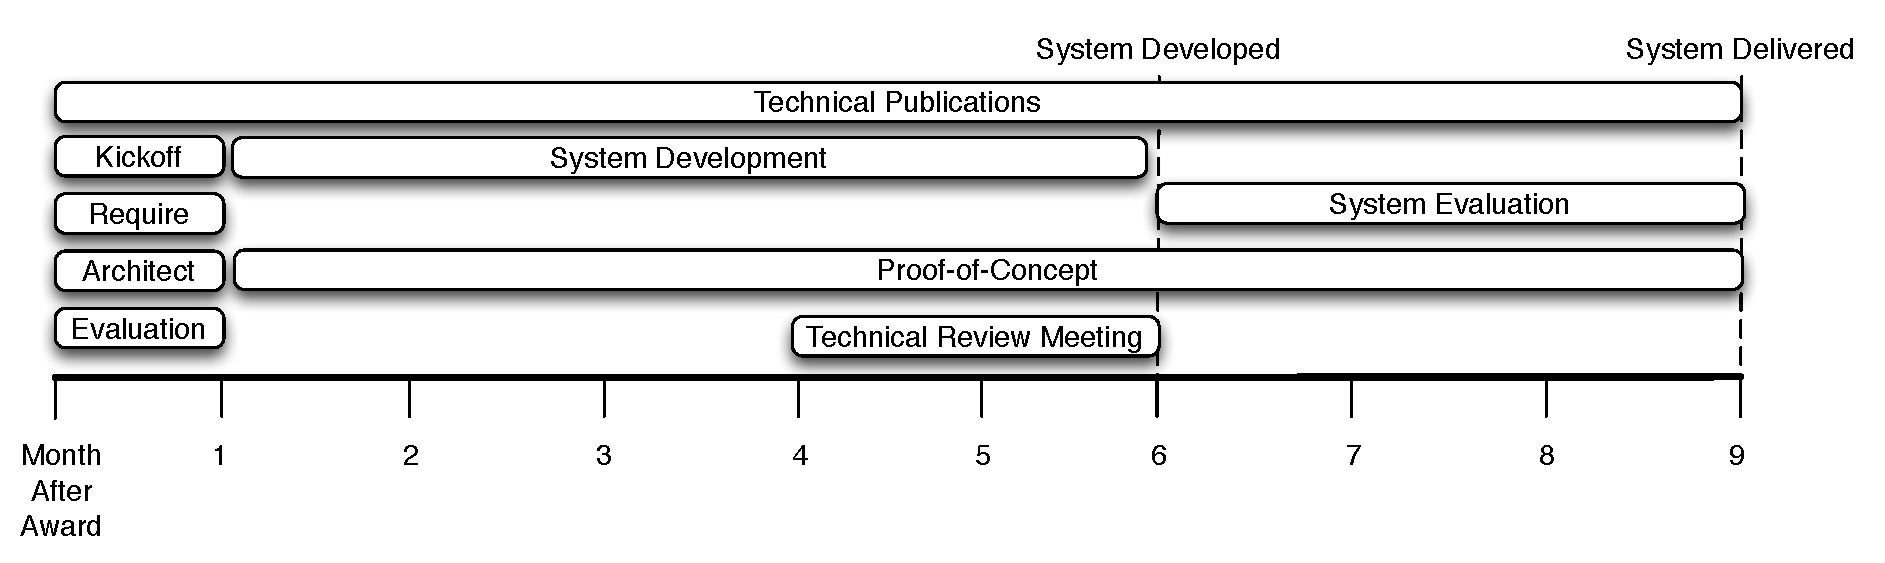
\includegraphics[width=\textwidth]{images/gantt.pdf}
\caption{The proposed project schedule.}
\label{fig:gantt}
\end{figure}

\subsection{Task Outline}
We expect to begin work via a kickoff meeting, followed by requirements analysis, development, and prototype delivery as shown in Figure~\ref{fig:gantt}.  During this first phase we will focus on a notional mission-critical system and aggregated services used within that application.  We will review progress with the customer regularly, preparing for future phase II work.
\begin{enumerate}

\vspace{-0.1in}
\item {\bf Kickoff Meeting}---We will conduct a meeting with the Sponsor POC within 30 days of contract start.
\item {\bf Requirements Extraction}---We will identify and enumerate system requirements.
\item {\bf Establish Approaches and Architectures}---We will develop a catalog of integration options to extend our NUBLU system including descriptions of the approaches and their advantages and disadvantages.
\item {\bf Evaluate System Architecture Options}---We will examine the integration options available and choose the most promising, as well as establish how a common extensible framework in which we can instantiate components embodying various approaches for future experimentation and comparison of different randomization parameters.
\item {\bf System Development}---We develop the randomization system and related functions.
\item {\bf System Evaluation}---We will test the developed system and measure key performance attributes.
\item {\bf Technical Review Meeting}---We will conduct a technical review within six (6) months of project start at a date and time to be coordinated with the Sponsor POC.
\item {\bf Proof-of-Concept Prototype}---We will develop a preliminary version of the CHAMELEON system as a proof-of-concept prototype demonstration.
\item {\bf Reports and Publications}---We will submit monthly progress reports and a final report (with SF 298).
\end{enumerate}

\subsection{Milestone Schedule}~\\
%The proposed Phase I effort is scheduled as shown in the Gantt chart in Figure~\ref{Gantt}. 
The majority of the primary research will be accomplished during the first six months of the Phase I SBIR project. The last three months will provide project continuity to Phase II. Work will be performed at AHS Engineering's  headquarters and at UNM's facilities in Albuquerque, New Mexico.

%Expected major tasking stretches over a nine month period, over three distinct technical tracks, integrating the tracks at the conclusion of Phase I. The first track involves implementing and showing the applicability of network address randomization over operational networks. This consists of specific subtasks addressing network randomization and multpath routing implementation over SDN. The second track involves DNS integration for accurate naming reflecting current address context. These tracks are then integrated into the NUBLU framework during the last three months of the project, providing continuity into Phase II. The third track stretches over the entire nine months and focuses on experimental evidence supporting various randomization parameters and constraints required to support operational quality-of-service levels.  All tasks are preceded by requirements gathering and architectural integration efforts, as outlined below.

%\begin{figure}[h]
% \centerline{\includegraphics[width=5in]{./images/Gantt.png}}
% \caption{Task and milestone schedule.}
% \label{Gantt}
%\end{figure}

\paragraph{Deliverables}

\begin{enumerate}[label=\alph*.] 
\vspace{-0.1in}
\item Kickoff meeting within 30 days of contract start.
\item Progress reports.
\item Technical review within 6 months.
\item Final report with SF 298.
\end{enumerate}

%Our work plan is fully responsive to the requirements stated in the AF131-039 topic. By producing a working proof-of-concept prototype, we will in fact achieve more than the requirements of the topic.

\newpage
\clearpage
\cfoot{\color{LeTigre}\vspace*{-1.25em}{\scshape\fromproposaltitle}~\\ \rm\thepage~\\ 
\it{Use or disclosure of data contained on this page is subject to the restriction on the first page of this volume.}}

\subsection{Phase I Work Plan}
{This Phase I SBIR will result in the definition of the CHAMELEON technical approach required to implement system components and algorithms, identifying risk associated with prototype development as well as an approach to quantify system performance.  These results will be in sufficient detail to show proof-of-concept and demonstrate feasibility for the Phase II project and Phase III commercialization.}

\subsubsection{Key Aspects and Innovation}
AHS Engineering is an experienced and highly capable SBIR/STTR contractor with a proven record of thorough research and innovation, directed toward solving real problems. AHS Engineering has been active for over a decade in researching the key technologies required in this effort. The University of New Mexico is an internationally recognized research institution, and the faculty members affiliated with this project are members of the Informatics Research Group, which is highly experienced in the areas of information security, data analytics, machine learning, and usage management. Our approach integrates proven existing technologies with new innovative approaches. The use and leverage of proven technology provides a sound foundation for our technical approach, reducing technical risk, and providing a platform for our key innovations.

\subsubsection{Task Summary and Schedule}
The proposed Phase I effort is organized into the tasks shown in Section~\ref{sec:tasks}.  Work will be performed at AHS Engineering's headquarters and at UNM facilities in Albuquerque, New Mexico.

\subsubsection{Task Details and Technical Approach}\label{sec:tasks}
The AHS Engineering team will follow an agile software development process for accomplishing the Phase I tasks detailed below. Agile promotes adaptive planning, evolutionary development and delivery, a time-boxed iterative approach, and encourages rapid and flexible response to change with a focus on delivering working software~\cite{La:03}. The below tasks describe the deliverables and timelines associated with each effort.

\paragraph{Task 1: Kickoff Meeting (month 1).}
We will hold a kickoff meeting either at the government's site or at AHS Engineering headquarters, in Albuquerque, New Mexico, based on Government Sponsor POC preference. In this meeting we will review the proposed technical approach and statement of work and clarify the research sponsor's technical direction. In order to begin to address specific system needs, the team will assemble a coarsely grained Concept of Operations document that describes how the CHAMELEON system should work. This will be a living document and will be updated regularly according to the agile process while the team executes other specific tasks. 

\paragraph{Task 2: Requirements Extraction (month 1).}
The CHAMELEON system has a wide requirements domain, stretching from network randomization to PKI inclusion and DNSSec extension. In this task, we will identify and enumerate system requirements, aiming for 90\% requirements coverage overall and 100\% requirements coverage with respect to core Phase I functionality. We will name and describe these requirements in a form suitable for future system development and documentation. This analysis will include identification of Sponsor POC scenarios of interest.

The primary deliverables from this task will be a document describing these requirements such that the requirements can be traced both forward into the actual system and backward to the initial requirements source. The requirements will be enumerated as well as presented in either use case or user story formats. We will also develop a lightweight Concept of Operations document to clarify expected functionality.

\paragraph{Task 3: Establish Approaches and Architectures (month 1).}
Network address randomization is a difficult, nuanced problem. A variety of established architectural patterns can be potentially brought to bear on the problem, but they need to be carefully evaluated to ensure they will provide the required levels of service and scalability. In this task, we will outline the potential architectural approaches we can use, describe how and why they are applicable, and address how they could be evaluated for potential prototypical use.

This task will result in the development of a catalog of architectural options including descriptions of the approaches and their advantages and disadvantages. This catalog will also include specific evaluation points and potential small proofs-of-concept that may be built into the CHAMELEON system.

\paragraph{Task 4: Evaluate System Architecture Options (month 1).}
Building on the catalog established in the previous tasks, we will evaluate outlined technical and architectural approaches with an eye towards identifying common features. We will examine the options available to us and choose the most promising as well as determine how we can establish a common extensible framework for CHAMELEON in which we can instantiate components embodying various different approaches for future experimentation and comparison.

The outcome of this task is an ordered listing of potential approaches and an architectural outline of a common framework for CHAMELEON in which we can test the approaches identified.

\paragraph{Task 5: System Development (months 2-6).}
In this task we will build a simple CHAMELEON framework based on the common architecture identified previously. We will keep the framework as simple as possible while highlighting key functionality. We will verify that these components can be loaded into the common CHAMELEON framework and run as expected so as to ease transition into future evaluation tasks. We will focus on actual randomization as a primary priority, de-emphasizing DNSSec extensions and IDS/IPS sensors for Phase I. We will also develop a simple prototype representational of specific randomization scenarios of interest to the Air Force consisting of multiple services to use a testbed for evaluating our approaches.

\paragraph{Task 6: System Evaluation (months 6-9).}
At this point in the project, we will have established the key CHAMELEON system components, developed the initial proof-of-concept technology, and will be prepared to evaluate various randomization approaches and techniques. In this task we will run the system and collect experimental results. During these experiments we will measure key performance attributes related to supportable system load, information delivery times, dropped messages, and randomization performance. 

\paragraph{Task 7: Technical Review Meeting (no later than month 6).}
We will hold a technical review meeting with the Government Sponsor POC within 6 months of project commencement. The CHAMELEON concept of operations, system requirements, and architectural options will be reviewed and refined at this meeting.

\paragraph{Task 8: Proof-of-Concept Prototype (months 2-9).}
We will develop a preliminary version of the CHAMELEON system as a proof-of-concept prototype demonstration. We will provide the demonstration using a representational mission-critical scenario, along with the software, design documents, test suites, and other supporting documentation.

\paragraph{Task 9: Reports and Publications (months 1-9).}
We will prepare monthly progress reports, the final technical report with SF 298, and the non-proprietary summary report, including all pertinent observations, nature of problems, positive as well as negative results, and design criteria established. We envision that one or more professional conference and journal papers will result from this research. With the customer's approval, we will publish the research results.

At the conclusion of this project, specific deliverables include requirements and operational concept documentation, an architectural catalog, software source code and related test suites, a prototype system, and experimental results as well as a final technical report. 

%The tasks outlined within this proposal identify specific deliverables the team will develop and submit to sponsoring organizations. Those specific deliverables include:
%\begin{itemize}
%\item {\bf Requirements}---A document listing identified requirements associated with requirement source organized both by list and context via use cases or user stories.
%\item {\bf Architectural Catalog}---A document describing system architectural options, advantages and disadvantages of those options, and how the they can be evaluated.
%\item {\bf Software Source Code}---Any and all developed source code, including proofs-of-concept and operational software. This will also include documentation of the developed software.
%\item {\bf Automated Test Suite}---An automated test suite covering the system and developed source code upon which the system is based at a to-be-determined level of test coverage.
%\item {\bf Prototype System}---The working prototype system itself, as well as the representational mission-critical scenario testbed. This will consist of operating system images, source code, and deployment instructions, as applicable.
%\item {\bf Experimental Results and Papers}---All experimental results and analysis, as well as any generated papers.
%\item {\bf Final Technical Report}---A report detailing the specifics of architectural evaluation activities, including information with respect to how the system operates, explanation of any design decisions made with supporting evidence, and guidance for future phase II activities.
%\end{itemize}

\sbirsection{Related Work}{
AHS Engineering Services is highly qualified to successfully perform this effort based on our directly related experience in DoD Intelligence, Surveillance, and Reconnaissance (ISR) systems, and with enabling technologies such as service-oriented architecture, net-centric computing, and cloud computing. The University of New Mexico's Informatics Laboratory is renowned for research in information security, information theory, and machine learning.}

\subsection{Co-Principal Investigators' Related Experience}
We propose Dr. Mark Heileman as AHS Engineering Services' Phase I Co-Principal Investigator (co-PI). Dr. Heileman has extensive experience as a research engineer and software system developer. His technological work has focused on applying artificial intelligence techniques and computer modeling to solve real-world business problems. Some of his early work in this area involved the practical application of expert systems and simulation modeling. More recently his work has involved the development of a trust evaluation framework for use in a layered sensing architecture that is intended to produce actionable situational awareness (the notion of trusted sensing is then built into the layered sensing architecture)~\cite{HeHeFiSt:09,HeHeHw:09}. He was recently the Co-PI on both the SMASHUP Phase II SBIR project and the Nublu Phase I STTR project. The SMASHUP research project resulted in the development of a formal framework that allows integration via mashups of content from various data sources in a secure manner~\cite{HeHeGiEv:10,HeHeShGiJa:11}. The Nublu research project delivered technological innovations to provide assured information sharing (AIS) capabilities using flexible cloud computing based architectures~\cite{HeHeNaLa:12}. A summary r\'esum\'e for Dr. Mark Heileman is provided in Section~\ref{Key_Personnel}.

We propose Dr. Gregory Heileman as CHAMELEON's Co-Principal Investigator(co-PI). Dr. Heileman has over twenty years of experience as a research scientist, and has published over one-hundred peer-reviewed journal articles and conference papers. His research interests are in the areas of information security and multimedia systems, the theory of computing and information, and machine learning. He serves on the Editorial Board for the International Journal of Multimedia Intelligence and Security. Dr. Gregory Heileman is considered an authority on information security and usage management ~\cite{Informatics}. Some of his early work in information security dealt with the development of secure container technology at the hardware level (see US Patent 6,731,756) \cite{PiHe:04}. His subsequent work has involved the development of architectural frameworks in support of access and usage control technologies \cite{HeJa:05,HeJaKhHr:07,JaHe:04,JaHeMa:06}, information forensics \cite{PeHeAb:07,QuPeHe:09}, and semantics-based information valuation \cite{AlHe:10,AlHe:08}. He was recently the Co-PI on the SMASHUP Phase II SBIR project and the Nublu Phase I STTR project; he will be a Co-PI on the ASW F2F Phase II STTR project. Dr. Gregory Heileman's experience is listed in Section~\ref{Key_Personnel}.

We propose Dr. Christopher Lamb as a Research Scientist. Dr. Lamb has extensive experience in software systems design and architecture, ranging in scale from embedded to internationally distributed software systems. Dr. Lamb's early work dealt with the control of heterogeneous cloud systems~\cite{LaJaHeAb:11} as well as specific programming languages that could more easily describe usage management semantics than current established standards~\cite{LaJaBoNaHe:11}. More recent work has addressed usage management concepts in cloud computing environments~\cite{JaLaHe:11,JaLaHe:12} as well as content-centric and overlay networks~\cite{LaHe:12b} and multi-level security domains~\cite{LaHe:12,LaHe:13}. Most recently, he has been active in studying the security of software defined networking and its application to secure computing systems. ~\cite{MENS:14}. Dr. Lamb's r\'esum\'e is included in Section~\ref{Key_Personnel}.

We propose Mr. Jeff Vettraino as a Principal Engineer. Jeff has extensive experience working with the DoD on various cloud and satellite related projects and products. A brief biography for Mr. Vettraino's is included in Section~\ref{subs}.

\subsection{AHS Engineering Services Related Work}
AHS Engineering Services is a research and development firm concentrating on the information needs of science and society. Our primary function is to discover and create new knowledge about scientific and technological topics for the purpose of uncovering and enabling development of valuable new products, processes, and services. We are focused on the need to understand, create, and apply new methods for modeling, managing, and acquiring information. As all aspects of science and society become increasingly information intensive, this need has never been greater. We have in-depth experience in the fields of Information Security (Crypto, Forensics, Usage Management, Trust Management and Privacy), Theory of Information (Information Theory, Algorithmic Game Theory, Learning Theory, Semantic Technology), and Information Architecture (Distributed Systems, Cloud Computing, Next Generation Internet Architectures, Cognitive Radio, Agent-based Systems, Trusted Computing Base).

Summarized below are the R\&D projects conducted by AHS Engineering Services that address the critical technologies that will enable successful CHAMELEON R\&D.

{\bf Green Wave: Assuring Trust between the Edges Phase I SBIR}---This project dealt with the problem of delivering universal situational awareness to decision makers, and in particular with the problem of providing a means of quantifying the ``trustworthiness'' of the various pieces of information contained within a layered sensing framework. Layered sensing is characterized by the appropriate sensor or combination of sensors/platforms, infrastructure and exploitation capabilities to generate that situation awareness and directly support delivery of ``tailored effects.'' During this research effort we created a prototype architecture that supported the gathering and propagating (both forwards, for decision making, and backwards, for post mortem analyses) of ``trust information'' computed at various nodes in a network. In addition, we computed trust metrics from this information that could be provided to a decision maker. \emph{In collaboration with Modus Operandi, Inc., Melbourne, FL. Contract completed January 2009. Customer: AFRL/RYTC, Mr. Jong Hwang. (937) 255-4709 x3591}.

{\bf SMASHUP: A Formal Framework for Secure Mashups Phase II SBIR}---The recent development of mashup technologies now enables users to easily collect, integrate, and display data from a vast array of different information sources available on the Internet. The ability to harness and leverage information in this manner provides a powerful means for discovering links between information, and greatly enhances decision-making capabilities. The availability of such services in a DoD environment will provide tremendous advantages to the decision-makers engaged in analysis of critical situations, rapid-response, and long-term planning scenarios. In this research project, we have developed a framework that will allow integration via mashups of content from various data sources in a secure manner. The framework is based on mathematical logic wherein data units are wrapped in policies that provide rules over the manner in which information is collected, aggregated, and rendered in different environments. An advantage of this approach is it provides a formal means for controlling the usage of resources within highly complex secure mashups. \emph{In collaboration with Modus Operandi, Inc., Melbourne, FL. Phase II Contract awarded May 2011. Customer: AFRL/RIEBB, Mr. Matthew Shaver. (315) 330-3295}.

\subsection{University of New Mexico Related Work}
Summarized below are the research projects conducted by the Informatics Research Laboratory at UNM that address the critical technologies that will enable successful CHAMELEON R\&D. As all aspects of science and society become increasingly information intensive, the need to understand, create, and apply new methods for modeling, managing, and acquiring information has never been greater. The UNM Informatics Lab, established by Professor Gregory Heileman, has considerable knowledge in the areas of information security, the theory of information, and information architectures.

{\bf Nublu: Assured Information Sharing in Clouds Phase I \& II STTR}---We are developing an assured information sharing framework for cloud-based systems that leverages our ongoing work in the areas of policy-based usage management and semantic interoperability. The development of this framework involved the creation of a novel approach to information sharing that treats security as a commodity that can be dynamically provisioned within the cloud, along with other cloud resources. Currently, the security of networked infrastructures tends to be managed statically. That is, security requirements are developed and implemented within the networking environment, and all of the information that traverses the network will have these hard-coded security policies applied to it. The research project addresses this issue by logically separating security policies from security implementations within the network using software defined networking techniques and technologies. This approach is vital if the true capabilities of the cloud are to be realized in DoD environments; it naturally meshes with the philosophy behind cloud computing. Specifically, the main advantage of cloud systems is the automatic provisioning of resources according to current demands. In a DoD setting there will be multiple missions currently interacting with the cloud infrastructure, and the proposed framework will allow each mission to do so according to the current security demands. \emph{In collaboration with Modus Operandi, Inc., Melbourne, FL. Phase II Contract awarded. Customer: AFRL/RITB, Dr. George Ramseyer. (315) 330-3492}.

{\bf Anti-Submarine Warfare Find-to-Forecast Phase I \& II STTR}---The ASW F2F Project is focused on extracting situational knowledge from unstructured data sources, specifically tactical communications between Seahawk helicopters and the carrier, to fuse with structured data, such as radar and sonar data. This has involved developing a mission ontology for ASW, building a vocabulary for missions, and building specialized grammars for text parsing, tagging, extraction, and normalization as RDF triples. \emph{In collaboration with Modus Operandi, Inc., Melbourne, FL. Phase I Contract awarded June 2011. Phase II Contract awarded. Customer: Office of Naval Research, Mr. David McGrane (360) 315-3531}.

{\bf Network Architecture and Security. Project Name: ``Collaborative Research: Transient Network Architecture,'' National Science Foundation} in collaboration with the Center for National Research Initiatives (CNRI), Reston, VA. This work involved the development of the Transient Network Architecture for the next generation Internet. Our work on this project involved investigating how the capabilities offered by the networking architecture would facilitate the management of content. Specifically, we considered how the rights expressed by rights expression languages (RELs) could be supported by emerging Internet infrastructures. We considered how the ability to effectively use RELs could be further supported by changes made to the Internet infrastructure. For example, the notion of adding ``rights awareness'' to routers and firewalls was considered, allowing rights models to be more effectively and less intrusively implemented within the infrastructure. In addition, we addressed the problem of location-based rights in current and future infrastructures. This involved the consideration of authorized domains that essentially use the IP addresses of machines in order to determine where the content can be used, along with a more natural implementation of this problem that used handles as identifiers. \emph{Project completed July 2008. National Science Foundation, Future Internet Design (FIND) Program, Darleen Fisher, (703) 292-8950.}

\subsection{Cohesive Integrations Related Work}
Cohesive Integrations has experience designing, developing and delivering production software deployments throughout the DoD and IC. Captured below are relevant efforts in which Cohesive Integrations has been involved in that focus on integrating software with existing DoD software and Systems. Cohesive Integrations has partnered with UNM and AHS on SMASHUP and NUBLU, mentioned previously.

{\bf DCGS Integration Backbone (DIB)}---Cohesive Integrations, has supported all phases of the software lifecycle for the DIB including supporting the deployment and integration of the DIB into Programs of Record (PoR) enterprise systems. Recently Cohesive Integrations supported Hanscom Air Force Base by serving as the Product Owner for the DIB 4.0.2 release, and a SME for the DIB 4.1 release. A large focus of this effort was the on Information Security/Assurance, including supporting PL3 and PL4 environments. Additionally, the Hanscom milCloud environment was used to rapidly deploy, test and verify the software. The milCloud environment allows systems to be repeatedly and continuously (if desired) configured, deployed and tested in a manner of minutes. These systems can consist of a single VM instance or a full enterprise deployment. \emph{Mark Murray, Lt Col, USAF (781)-225-0677.}

\sbirsection{Relationship with Future Research or Research and Development}{}
Phase I will demonstrate the feasibility of our approach and will lay the groundwork for Phase II development and transition. Our Phase I work will create a limited prototype demonstrating how we intend to implement network address randomization via COTS hardware, including triage and replacement of suddenly untrusted services, PKI, and secure naming. That prototype will support network randomization, service motion, enclave creation and management, and encryption capabilities. We will conduct the needed groundwork to prepare for secure naming and specific address and path randomization algorithms for Phase II. In Phase II, we will build the full CHAMELEON randomization system, incorporating it with operational mission-critical applications to demonstrate appropriate service obfuscation. Our successful realization of our Phase I and II objectives and achievement of Phase III commercialization is expected to provide the following benefits to both Government and private sector customers:

\vspace{-0.1in}
\begin{itemize}
     \item Enhanced cyber-security posture for sensitive systems.
     \item Included PKI capability.
     \item Rapid secure enclave setup and teardown.
     \item Authenticated and confidential naming based on DNSSec.
\end{itemize}

We are confident of our ability to successfully deliver these benefits. As for future R\&D, we will seek out ways to extend the scope of CHAMELEON to more complex computational environments incorporating more clients and mobile devices.

\sbirsection{Commercialization Strategy}{Our overall strategy for achieving technology transition and commercialization success will be to apply the CHAMELEON framework to federal transition customers while making our technology available and known to commercial cloud and datacenter operators.}
\label{commercialization}
AHS Engineering Services will collaborate with the Innovate ABQ initiative that was recently established in the City of Albuquerque as a premier innovation district that brings together the research power of the state's flagship university with Albuquerque's entrepreneurial and established business community to create new companies and business opportunities. The City of Albuquerque, the University of New Mexico and other entities have invested more than \$6 million in this initiative.  

We will have access to the services provided by Innovate ABQ and are committed to using this to further the commercialization potential of this research. We anticipate that his will include marketing expertise, access to venture capitalists, along with collaborative work spaces, among other benefits. A letter of support from the City of Albuquerque's Director of Economic Development, and a leader in the Innovate ABQ effort, is attached.

\paragraph{Market Need and Size.} We have identified two key market segments to our plans for commercialization of CHAMELEON. Those market segments are data center operators and cloud computing providers, both of which are briefly described below. We intend to capitalize on the market timing generated by the current convergence of these key market segments.

We developed our NUBLU technology atop and within the OpenDaylight SDN controller ecosystem~\cite{opendaylight}. This controller framework is widely deployed in SDN-capable controller environments today, and is supported by all major network equipment vendors. We intend to make our technology available as plugins and extensions to this framework. This gives us an immediate commercialization channel into the vast majority of software defined networks deployed today. Furthermore, as organizations upgrade network hardware, more and more networks will support SDN, and the potential market will grow. Ancilliary technologies like Docker are capturing additional market as well, and have similar support from major vendors~\cite{docker}.

\vspace{-12pt}
\subparagraph{Data Center Operators.} Data center operators would not generally need the ability to quickly create securable enclaves, but could use address space randomization internally to heighten overall cyber-security posture. This kind of randomization could in fact be implemented such that while key systems may have externally accessible IP addresses, the majority of systems providing internal services are completely randomized and only accessible via secured naming services that provide up-to-date host address resolution. The global data center operator market is expected to over \$20 billion by 2018~\cite{datacentermarket}.

\vspace{-12pt}
\subparagraph{Cloud Computing Providers.} Cloud computing providers with data center infrastructure access can use all the functionality we are proposing. They can quickly and easily create secure enclaves (which are, in fact very similar to virtual private clouds, but with more security and enhanced virtualized network functions). We have worked closely with the milCloud team at Hanscom AFB in the scope of our NUBLU work and will continue to do so to help bring immediate return on this investment. The cloud computing market is currently over \$131 billion in size~\cite{cloudmarket}.

\paragraph{Projected Commercialization Results.} Our commercialization strategy consists of two paths:

\vspace{-18pt}
\subparagraph{Our first path} focuses on transitioning the technology thereby providing direct return-on-investment for SBIR investment. Our existing knowledge and experience working with other federal customers will provide a solid foundation for success in this initiative. Our ability to leverage the market penetration of the OpenDaylight controller framework also gives is immediate access into both government and commercial organizations.

\vspace{-18pt}
\subparagraph{Our second path} involves deployment in support of other government customers and prime contractors.  Our initial focus for this part of our overall strategy will be to leverage our current relationships with milCloud development staff and familiarity with their overall roadmap. The technologies we use are currently planned for integration within the milCloud environment within the next one to two years, providing robust infrastructure for CHAMELEON deployment on a timeline that meshes well with this SBIR development timeline.

The timeline and expected funding for commercialization are:
\vspace{-18pt}
\subparagraph{Year 1:} SBIR Phase I funding of \$150,000 for concept feasibility and refinement. No additional capital expected.
\vspace{-18pt}
\subparagraph{Years 2--3:} SBIR Phase II funding of \$750,000 for concept development for interested federal customers (i.e., relevant environment). Anticipated additional customer capital of \$50,000--500,000 obtained to enhance the CHAMELEON design.
\vspace{-18pt}
\subparagraph{Year 4:} SBIR Phase III rollout of CHAMELEON, funded by customer capital raised according to needs. Anticipated customer capital of \$1--5 million obtained to provide sensitive information management for a program of record (POR).

\sbirsection{Key Personnel}{All key personnel are United States citizens.}
\label{Key_Personnel}
We propose Dr. Mark Heileman as the Phase I Co-Principal Investigator, along with Dr. Gregory Heileman, with technical assistance provided by Dr. Christopher Lamb, and Mr. Jeff Vettraino.  Dr. Heileman's, Dr. Lamb's, and Dr. Gregory Heileman's biography and r\'esum\'es are below. Mr. Jeff Vettraino's r\'esum\'e is in Section~\ref{subs}.
\vspace{-0.1in}
\begin{center}
    \fcolorbox{BlueSteel}{Magnum}{
         \begin{minipage}[t]{0.9\textwidth}
             \begin{itemize}[labelindent=2em,leftmargin=1.5em,label=$\checkmark$]
  		\item Dr. Mark Heileman has extensive experience as a research engineer and software system developer. He has focused on applying advanced information technology and modeling to solve real-world business problems.
  		\item Dr. Gregory Heileman is is a recognized leader in neural networks and policy-based information processing.  
		\item Dr. Christopher Lamb  is a TOGAF certified enterprise architect and a Certified Information Systems Security Professional. An experienced software engineer, he is actively engaged in cyber-security research.
		\item Mr. Jeff Vettraino is a core engineering leader for various Air Force satellite and cloud computing efforts.
 	\end{itemize}
         \end{minipage}
      }
\end{center}

\vspace{-6pt}
{\bfseries Dr. Mark Heileman's over thirty-year career includes engineering and executive positions with Elisar Software Corporation, i2 Technologies, United Space Alliance, Rockwell International, and Harris Corporation. He has been the PI on six SBIR/STTR projects at MO.}

\textbf{\textsc{Mark D. Heileman \hfill Scientist}}

\vspace{-18pt}
{\textcolor{black}{\makebox[6.5in]{\hrulefill}}
\textbf{\textsc{Technical Expertise:}}
\vspace{-8pt}
\begin{multicols}{2}
 \begin{itemize}
  \item Enterprise Information Systems
  \item Digital Rights Management
  \item Cyber Security
  \item Expert Systems
  \item Data Aggregation
  \item Simulation and modeling	
 \end{itemize}
\end{multicols}
\vspace{-16pt}
\textbf{\textsc{Selected Publications:}}
\vspace{-8pt}
\begin{enumerate}
\item M. Heileman, G. Heileman, M. Shaver, P. Jamkhedkar, and M. Gilger. SMASHUP: Secure Mashup for Defense Transformation and Net-Centric Systems. {\sl SPIE Defense, Security, and Sensing 2011 Conference}, Orlando, FL, 25--29 April 2011.
\item G. Heileman and M. Heileman. Method and Apparatus for Integrating Subjective Trust Measures into Automated Decision-Making Processes. Provisional Patent Application, USA, submitted 19 May 2010.
\item M. Heileman, G. Heileman, and J. Hwang. Integrating Subjective Trust into Networked Infrastructures. {\sl Systems \& Software Technology Conference (SSTC) 2009}, Salt Lake City, UT, 20--23 April 2009.
\item R. Hull, K. Bimson, M. Heileman, R. Hyle, and R. Thiebauth. Semantic Service-Oriented Architecture for Range Operations: Evolving the Role of Semantics in the Enterprise. {\sl SPIE Defense, Security, and Sensing 2009 Conference}, Orlando, FL, 13--17 April 2009.
\item H. Goldstein, G. Heileman, M. Heileman, et al. Protecting Digital Archives at the Greek Orthodox Archdiocese of America. {\sl DRM'03}, Washington, DC, 27 October 2003.
\item D. Linton, S. Khajenoori, M. Heileman, J. Bullington, H. Cat, K. Halder, G. Hebert, and S. Sinnappan. ``Reporter Object: An Analysis Module Which Aids in Verifying, Validating and Graphically Displaying Results of Simulation Models,'' {\sl Simulation}, Vol. 62, No. 5, May 1994, pp. 313--328.
\item M. Heileman, D. Linton, and S. Khajenoori. ``Simulation Study Aids Space Shuttle Flight Rate Planning,'' {\sl Industrial Engineering}, Vol. 24, No. 3, March 1992, pp. 58--59.
\end{enumerate}

\vspace{-6pt}
\textbf{\textsc{Relevant Experience:}}~\\
{\bfseries AHS Engineering Services, 2014--present.} Project Manager. A research and development firm offering expert engineering services in areas including software engineering and information security.~\\
{\bfseries University of New Mexico, Department of Electrical \& Computer Engineering, 2013-- present.} Research Professor.~\\
{\bfseries Modus Operandi, Inc., 2004--2014.} Scientist. A software company serving the US defense and intelligence community by providing technology to speed information discovery, integration, and fusion. Directs the design and development of innovative information system technologies and their application to government and industry needs.~\\
{\bfseries Elisar Software Corporation, 2001--2003.} Vice President, Sales Engineering. A venture capital financed start-up software company providing digital rights enforcement products and services. Initiated the Sales Engineering function, which had primary responsibility for driving customer and market requirements into the internal development process.~\\
{\bfseries i2 Technologies, 1997--2001.} Senior Solution Consultant. A business software and services company providing supply chain management solutions to customers worldwide. Provided technical leadership throughout software products sales cycles.

\vspace{-12pt}
\textbf{\textsc{Education:}}
\vspace{-29pt}
\begin{tabbing}*****************\=\kill
 \> {\bfseries Ph.D.}, Industrial Engineering \& Management Systems, Univ. of Central Florida (1997). \\
 \> {\bfseries M.S.}, Engineering Management, Florida Institute of Technology (1990). \\
 \> {\bfseries M.B.A.}, Business Administration, Florida Institute of Technology (1985). \\
 \> {\bfseries B.S.}, Industrial and Systems Engineering, University of Florida (1980).
\end{tabbing}

\vspace{-12pt}
\textbf{\textsc{Affiliations:}}
\vspace{-30pt}
\begin{tabbing}*****************\=\kill
\> Registered Professional Engineer, State of Florida (P.E. \#35539). \\
\> Senior Member, Institute of Industrial Engineers. \\
\> Member, International Council on Systems Engineering (INCOSE). \\
\> Security Clearance: DoD Top Secret/SCI (inactive).
\end{tabbing}


\textbf{\textsc{Gregory L. Heileman \hfill Professor and Associate Provost}}

\vspace{-18pt}
{\textcolor{black}{\makebox[6.5in]{\hrulefill}} 
\textbf{\textsc{Technical Expertise:}}
\vspace{-8pt}
\begin{multicols}{2}
 \begin{itemize}
  \item Machine Learning
  \item Usage Management
  \item Information Security
  \item Data Structures and Algorithmic Analysis
  \item Theory of Computing and Information        
 \end{itemize}
\end{multicols}

\vspace{-16pt}
\textbf{\textsc{Selected Publications:}}
\vspace{-8pt}
\begin{enumerate}
\item C.~C. Lamb and G.~L. Heileman. Content-centric Information Protection in the Cloud, {\sl International Journal of Cloud Computing and Services Science  (IJ-CLOSER)}, 2(1):246-257, 2013.

\item P. A. Jamkhedkar, C. C. Lamb, and G. L. Heileman. Usage Management in Cloud Computing, In F. Hartung, T. Kalker and S. Lian, Eds., {\sl Digital Rights Management: Technology, Standards and Applications}, Auerbach Publications, 2012. 

\item C. C. Lamb, P. A. Jamkhedkar, G. L. Heileman and C. T. Abdallah. Managed Control of Composite Cloud Systems. 6th IEEE International Conference on System of Systems Engineering (SoSE), Albuquerque, NM, pp. 167--172, June 27--30, 2011.

\item P.~A. Jamkhedkar and G.~L. Heileman. Rights Expression Languages, in S. Lian and Y. Zhang, Eds., {Handbook of Research on Secure Multimedia Distribution}, IGI Global, Hershey, PA, 2008.
 
\item S. al-Saffar and G. L. Heileman. Computing Information Value from RDF Graph Properties. Proceedings of the 12th International Conference on Information Integration and Web-based Applications \& Services, Paris, Nov. 8--10, 2010.

\item T.-T. Quach F. Perez-Gonzalez, and G. L. Heileman. Model-Based Steganalysis Using Invariant Features. IS\&T/SPIE Electronic Imaging Science and Technology: Media Forensics and Security XI (Conference EI120), San Jose, CA, Jan. 18--22, 2009.

\item S. al-Saffar and G. L. Heileman. Semantic Impact Graphs for Information Valuation. Proceeding of the Eighth ACM Symposium on Document Engineering, Sao Paulo, Brazil, pp. 209--212, Sept. 16--19, 2008.

\item S. al-Saffar and G. L. Heileman. Semantics-Based Information Valuation. Proceedings of the 4-th IEEE International Conference on Intelligent Systems IS'08, Varna, Bulgaria, Vol. 1, pp. 6-51--6-58, Sept. 6--8, 2008.

\end{enumerate}

\vspace{-6pt}
%\fxnote{AHS no longer a consulting firm.}
\textbf{\textsc{Relevant Experience:}}~\\
{\bfseries AHS Engineering Services, 1997--present. Principal.} A firm offering expert engineering services in areas including software engineering and information security.~\\
{\bfseries University of New Mexico, Department of Electrical \& Computer Engineering, 1990--present. Professor, Associate Provost for Curriculum (current position)}.~\\
{\bfseries Elisar Software Corporation, 2000--2003. Chief Executive Officer and Chairman of the Board.} A venture capital financed start-up software company providing digital rights enforcement products and services.

\vspace{-6pt}
\textbf{\textsc{Education:}}
\vspace{-30pt}
\begin{tabbing}*****************\=\kill
 \> {\bfseries Ph.D.}, Computer Engineering, University of Central Florida (1989). \\
 \> {\bfseries M.S.}, Biomedical Engineering \& Mathematics, University of North Carolina (1986). \\
 \> {\bfseries B.A.}, Biology, Wake Forest University (1982).
\end{tabbing}

\vspace{-12pt}
\textbf{\textsc{Affiliations:}}
\vspace{-30pt}
\begin{tabbing}*****************\=\kill
\> Editorial Board,  International Journal of Multimedia Intelligence and Security. \\
\> Senior Member, IEEE. \\
\> Security Clearance: DoD Secret.
\end{tabbing}
\vspace{-12pt}

\textbf{\textsc{Christopher C. Lamb \hfill Research Professor / Principal Scientist}}

\vspace{-18pt}
{\textcolor{black}{\makebox[6.5in]{\hrulefill}}
\textbf{\textsc{Technical Expertise:}}
\vspace{-8pt}
\begin{multicols}{2}
\begin{itemize}
 \item Software Defined Networking
 \item Network Functions Virtualization
 \item Cloud Systems Security
 \item Systems and Software Architecture
 \item Software Engineering and Design
 \item Next-Generation Software Systems Security	
\end{itemize}
\end{multicols}

\vspace{-16pt}
\textbf{\textsc{Selected Publications:}}
\begin{enumerate}
\item Christopher Lamb and Gregory Heileman.
\newblock Content-centric information protection in cloud computing.
\newblock {\em International Journal of Cloud Computing and Services Science}, 2(1):246--257, 2012.

\item Christopher~C. Lamb, Pramod~A. Jamkhedkar, and Gregory~L. Heileman.
\newblock {\em Digital Rights Management: Technology, Standards and Applications}.
\newblock Auerbach Publications, 2013.

\item C.C. Lamb and G.L. Heileman.
\newblock Overlay architectures enabling cloud computing for multi-level security environments.
\newblock In {\em Services (SERVICES), 2012 IEEE Eighth World Congress on}, pages 116 --124, june 2012.

\item Christopher~Charles Lamb, Pramod~A. Jamkhedkar, Mathew~P. Bohnsack, Viswanath Nandina, and Gregory~L. Heileman.
\newblock A domain specific language for usage management.
\newblock In {\em Proceedings of the 11th annual ACM workshop on Digital rights management}, DRM '11, pages 51--62, New York, NY, USA, 2011. ACM.

\item Christopher~C. Lamb, Pramod~A. Jamkhedkar, Gregory~L. Heileman, and Chaouki~T. Abdallah.
\newblock Managed control of composite cloud systems.
\newblock In {\em System of Systems Engineering (SoSE), 2011 6th International Conference on}, pages 167 --172, June 2011.

\item P.A. Jamkhedkar, C.C. Lamb, and G.L. Heileman.
\newblock Usage management in cloud computing.
\newblock In {\em Cloud Computing (CLOUD), 2011 IEEE International Conference on}, pages 525 --532, july 2011.

\item Pramod~A. Jamkhedkar, Gregory~L. Heileman, and Chris~C. Lamb.
\newblock An interoperable usage management framework.
\newblock In {\em Proceedings of the tenth annual ACM workshop on Digital rights management}, DRM '10, pages 73--88, New York, NY, USA, 2010. ACM.
\end{enumerate}

\vspace{-6pt}
\textbf{\textsc{Relevant Experience:}}~\\
{\bfseries University of New Mexico, Department of Electrical \& Computer Engineering, 2013--present.} Research Professor.~\\
{\bfseries Sandia National Laboratories, 2004--present.} Principal Scientist. Architecture development and security analysis; ICAM architectures; heterogeneous analytic component systems engineering; program development; micro-controller engineering (PIC32, PIC16); service-oriented system architecture, design, and development; software engineering; general project management.~\\
{\bfseries Oso Grande Technologies, 2001--2004.} Vice President, Software Engineering. Led a multi-disciplinary team brokering information via web services between national insurance aggregators and state governments; responsible for profitability, business development, technical architecture and development.

\vspace{-6pt}
\textbf{\textsc{Education:}}
\vspace{-30pt}
\begin{tabbing}*****************\=\kill
\> {\bfseries Ph.D.}, Computer Engineering, University of New Mexico (2012). \\
\> {\bfseries M.S.}, Computer Science, University of New Mexico (2002). \\
\> {\bfseries B.S.}, Mechanical Engineering, New Mexico State University (1994).
\end{tabbing}

\vspace{-12pt}
\textbf{\textsc{Affiliations:}}
\vspace{-30pt}
\begin{tabbing}*****************\=\kill
\> Member, IEEE. \\
\> Security Clearance: DoE Q.
\end{tabbing}

\sbirsection{Foreign Citizens}{}
We do not expect to involve any foreign citizens on this project.

\sbirsection{Facilities/Equipment} {}
All instrumentation and physical facilities required to carry out the Phase I effort are available at AHS and the University of New Mexico campus in Albuquerque, NM. All project key personnel have dedicated laptop computers with high-speed network connections.  UNM also has a dedicated cloud laboratory in which we will deploy any required software.  No items of equipment are to be purchased for the Phase I effort. These facilities meet all environmental laws and regulations of federal, New Mexico, and local governments for, but not limited to, the following groupings: airborne emissions, waterborne effluents, external radiation levels, outdoor noise, solid and bulk waste disposal practices, and handling and storage of toxic and hazardous materials.

\sbirsection{Subcontractors/Consultants}{}
\label{subs}
Mr. Vettraino, the Chief Technology Officer of Cohesive Integrations, specializes in the design, development and rapid deployment of distributed, web-based software geared towards secure data discovery and dissemination, particularly for the DoD/IC. He is experienced in full software life-cycle development from inception to deployment and maintenance, as well as ensuring the security of data from creation to dissemination to end user systems and/or devices. His recent work with different software technologies and programs leveraging Hanscom milCloud have proven an effective way to develop and test software designed to operate in a realistic DoD cloud environment, while minimizing time and cost.

\vspace{-12pt}

\sbirsection{Prior/Current/Pending Support of Similar Proposals/Awards}{}
No prior, current, or pending support for the proposed work.

\printbibliography

\clearpage

%\include{images/innovate-abq-letter.pdf}

\begin{figure}[!t]
\centering

\includegraphics[width=\textwidth]{images/innovate-abq-letter.pdf}
%\caption{The overall concept of operations of the CHAMELON system, highlighting enclave creation, from a logical perspective.}
%\label{fig:conops}
\end{figure}

\end{document}
